\documentclass[11pt,a4paper]{article}

% --- Page / typography ---
\usepackage[a4paper,margin=2.5cm]{geometry}
\usepackage[T1]{fontenc}
\usepackage[utf8]{inputenc}
\usepackage{lmodern}
\usepackage{microtype}
\usepackage{setspace}
\setstretch{1.1}

% --- Math / Physics ---
\usepackage{amsmath}
\usepackage{amssymb}
\usepackage{bm}

% --- Graphics / Diagrams ---
\usepackage{tikz}
\usetikzlibrary{shapes, arrows.meta, positioning, patterns, decorations.pathmorphing, shadows}
\usepackage{float}
\usepackage{caption}
\captionsetup{font=small,labelfont=bf}

% --- Nice rules / boxes ---
\usepackage{tcolorbox}
\tcbset{colback=gray!5,colframe=black!20,boxrule=0.6pt,arc=3pt,left=10pt,right=10pt,top=8pt,bottom=8pt}

% --- Header / footer ---
\usepackage{fancyhdr}
\pagestyle{fancy}
\fancyhf{}
\lhead{\small \textbf{Generalized Universe Holography (GUH)}}
\rhead{\small Version 0.2 | 4 Jan 2026}
\cfoot{\small \thepage}
\renewcommand{\headrulewidth}{0.5pt}

% --- Title styling ---
\usepackage{titlesec}
\titleformat{\section}{\large\bfseries}{\thesection.}{0.6em}{}
\titleformat{\subsection}{\normalsize\bfseries}{\thesubsection.}{0.6em}{}

% --- Metadata Links ---
\usepackage[hidelinks]{hyperref}
\usepackage{url}

% --- Document Info ---
\newcommand{\papertitle}{GENERALIZED UNIVERSE HOLOGRAPHY (GUH)}
\newcommand{\papersubtitle}{A Working Hypothesis}
\newcommand{\authorname}{Alliance Research Group (ARG)}
\newcommand{\collab}{Collaborative Human-AI Exploration}
\newcommand{\credits}{(Distilled by Grok, Gemini, and OpenAI-inspired insights)}
\newcommand{\version}{0.3}
\newcommand{\docdate}{4 January 2026}
\newcommand{\license}{Open Access -- Attribution Required}

\begin{document}

% --- Title Page Block ---
\begin{center}
    \vspace*{0.5cm}
    {\Huge\bfseries \papertitle \par}
    \vspace{0.3cm}
    {\Large \papersubtitle \par}
    \vspace{0.8cm}
    
    {\normalsize
    \textbf{\authorname} \\
    Łukasz ``Captain'' Bojanowski \\
    \textit{\collab} \\
    \footnotesize \credits \par
    }
    
    \vspace{0.5cm}
    {\small
    \textbf{Date:} \docdate \quad \textbf{Version:} \version \\
    \textbf{Status:} Working Hypothesis (Non-Dogmatic / Falsifiable) \\
    \textbf{License:} \license
    }
\end{center}

\vspace{0.8cm}

% --- DEDICATION ---
\begin{center}
    \begin{minipage}{0.8\textwidth}
        \centering
        \itshape
        Dedicated to the memory of the late Professor Kazimierz Musiał (1994-1997),\\
        my high school physics teacher.\\
        \vspace{0.2cm}
        This work would not have come into existence without the inspiration and passion\\
        he instilled in me decades ago.
    \end{minipage}
\end{center}
\vspace{0.8cm}
\hrule
\vspace{0.8cm}

% --- Abstract ---
\section*{Abstract}
The Generalized Universe Holography (GUH) hypothesis extends the holographic principle beyond Anti-de Sitter (AdS) spaces to describe our observed flat or de Sitter-like universe. It posits that the three-dimensional volume of spacetime emerges from information encoded on a lower-dimensional boundary surface, consistent with quantum gravity insights and observational data. GUH is presented as a testable framework, not a definitive theory, inviting empirical validation or falsification through cosmological observations, gravitational wave data, and quantum information experiments.

\vspace{0.3cm}
\noindent \textbf{Keywords:} holographic principle, quantum gravity, cosmology, black hole information, emergent spacetime

\tableofcontents
\newpage

% --- CONTENT ---

\section{Introduction}
The holographic principle, first proposed by 't Hooft (1993) and Susskind (1995), states that the description of a volume of space can be encoded on its boundary surface, with information density bounded by the surface area rather than volume. This idea, formalized in the AdS/CFT correspondence by Maldacena (1998), has profoundly influenced quantum gravity research.

GUH generalizes this principle to cosmologies beyond AdS, including our observed $\Lambda$CDM universe. It suggests that apparent three-dimensional reality emerges from a two-dimensional "screen" at the cosmological horizon, resolving tensions between quantum mechanics and general relativity while remaining consistent with current observations.

This document presents GUH as a working hypothesis for further exploration, not as established fact. Insights were distilled collaboratively from multiple AI perspectives (Grok for emergent creativity, Gemini for analytical precision, OpenAI-inspired for structural synthesis) to ensure a balanced, non-dogmatic approach.

\section{Foundations of the Holographic Principle}

\subsection{Black Hole Thermodynamics}
Bekenstein (1973) and Hawking (1975) showed that black hole entropy is proportional to horizon area:
\begin{equation}
    S = \frac{k c^3 A}{4\hbar G}
\end{equation}
where $A$ is horizon area, $k$ Boltzmann's constant, $c$ speed of light, $\hbar$ reduced Planck's constant, and $G$ gravitational constant. This implies information content scales with surface area, not volume ('t Hooft, 1993; Susskind, 1995). Mathematically, the entropy bound for a region of space is $S \le (A/4)$ in Planck units, suggesting holographic encoding.

\subsection{AdS/CFT Correspondence}
Maldacena (1998) demonstrated exact duality between gravity in Anti-de Sitter space (AdS) and conformal field theory (CFT) on its boundary, providing mathematical evidence for holography in curved spacetimes. The duality is expressed as:
\begin{equation}
    Z_{AdS} = Z_{CFT}
\end{equation}
where $Z$ is partition function, linking bulk gravity to boundary quantum field theory.

\subsection{Extensions to Flat and de Sitter Space}
Recent work explores holography in cosmologically relevant spaces:
\begin{itemize}
    \item \textbf{Celestial holography} (Pasterski et al., 2023) for flat spacetime, where asymptotic symmetries map to 2D CFT on celestial sphere.
    \item \textbf{dS/CFT proposals} for de Sitter-like universes (Strominger, 2001; updated models 2024-2025), with entropy scaling as $S_{dS} \sim (A / 4G)$, where $A$ is cosmological horizon area.
\end{itemize}

\section{Related Work}
GUH builds upon and extends several key developments in holographic quantum gravity and cosmology:
\begin{itemize}
    \item \textbf{AdS/CFT Correspondence} (Maldacena, 1998): The most rigorous example of holography, providing an exact duality in negatively curved (AdS) spacetimes. GUH generalizes this to flat and de Sitter cosmologies.
    \item \textbf{Celestial Holography} (Pasterski et al., 2023): Proposes holography in asymptotically flat spacetimes. GUH shares the goal but emphasizes cosmological horizons as the relevant boundary.
    \item \textbf{dS/CFT and de Sitter Holography}: Explores holography in positively curved spaces. GUH incorporates elements of dS holography but focuses on emergent boundary encoding compatible with observations.
    \item \textbf{Holographic Dark Energy Models}: Treat dark energy as arising from holographic entropy bounds. GUH views dark energy as an emergent effect of boundary information evolution.
\end{itemize}

\section{Generalized Universe Holography (GUH) Hypothesis}
GUH proposes:
\begin{enumerate}
    \item The observable universe's degrees of freedom are encoded on a lower-dimensional boundary (cosmological horizon or similar surface).
    \item Three-dimensional spacetime and matter fields emerge from quantum entanglement and information processing on this boundary.
    \item Gravitational dynamics (including dark energy effects) arise from boundary quantum information evolution.
\end{enumerate}

GUH remains consistent with $\Lambda$CDM cosmology parameters (Planck Collaboration, 2020), Gravitational wave observations, and Black hole imaging (EHT).

\subsection{Mathematical Formulation}
In GUH, the entropy of a cosmological region is bounded by its boundary area:
\begin{equation}
    S \le \frac{A}{4l_P^2}
\end{equation}
where $l_P$ is Planck length. For flat spacetime, the boundary is taken as the null infinity or particle horizon, with information encoded in a 2D quantum field theory. The emergent metric satisfies:
\begin{equation}
    ds^2 = g_{\mu\nu}dx^{\mu}dx^{\nu}
\end{equation}
where $g_{\mu\nu}$ derives from boundary CFT correlators via duality similar to AdS/CFT, but generalized to flat space.

For de Sitter space, GUH extends dS/CFT with entropy:
\begin{equation}
    S_{dS} = \frac{3\pi}{G\Lambda}
\end{equation}
where $\Lambda$ is cosmological constant, linking to holographic dark energy models.

\section{Testable Predictions and Validation Paths}
GUH generates falsifiable predictions:
\begin{itemize}
    \item Specific patterns in cosmic microwave background (CMB) power spectrum beyond standard $\Lambda$CDM (potential anomalies in large-scale modes).
    \item Subtle deviations in gravitational wave propagation from distant mergers.
    \item Information-theoretic constraints on cosmological evolution.
\end{itemize}

\textbf{Suggested Validation Paths:} Analysis of CMB data for holographic signatures; Gravitational wave template modifications; Quantum information experiments probing entanglement structure.

\section{Limitations and Criticism}
GUH faces challenges in precisely defining the boundary in flat or de Sitter spacetimes, where the cosmological horizon is observer-dependent. Critics note that while AdS/CFT is mathematically rigorous, extensions to realistic cosmologies remain speculative. The hypothesis is explicitly presented as a working hypothesis open to revision or rejection based on future data.

\section{Research Roadmap}
\begin{itemize}
    \item \textbf{Short-term (2026–2027):} Analysis of upcoming CMB data (Euclid, CMB-S4).
    \item \textbf{Medium-term (2027–2030):} Quantum simulation of boundary CFT using near-term quantum devices.
    \item \textbf{Long-term:} Integration with candidate quantum gravity theories and multi-messenger tests.
\end{itemize}

\section{Visual Representations}
Conceptual diagrams illustrating key aspects of GUH.

% --- DIAGRAMS ---
\begin{figure}[H]
    \centering
    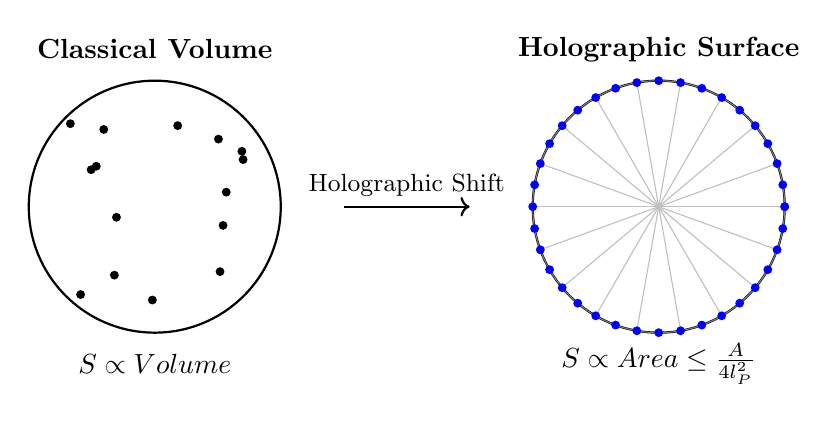
\begin{tikzpicture}[scale=0.8]
        % Classical
        \draw[thick] (0,0) circle (2cm);
        \node at (0,2.5) {\textbf{Classical Volume}};
        \foreach \i in {1,...,15} \fill[black] (rand*1.5, rand*1.5) circle (2pt);
        \node at (0,-2.5) {$S \propto Volume$};
        
        \draw[->, thick] (3,0) -- (5,0) node[midway, above] {\small Holographic Shift};

        % Holographic
        \begin{scope}[xshift=8cm]
            \draw[thick] (0,0) circle (2cm);
            \draw[gray, thin] (0,0) circle (2cm);
            \foreach \a in {0,20,...,360} \draw[gray!50] (0,0) -- (\a:2cm);
            \node at (0,2.5) {\textbf{Holographic Surface}};
            \foreach \a in {0,10,...,360} \fill[blue] (\a:2cm) circle (2pt);
            \node at (0,-2.5) {$S \propto Area \le \frac{A}{4l_P^2}$};
        \end{scope}
    \end{tikzpicture}
    \caption{\textbf{Entropy Bound Comparison.} Information encoding shifting from volume to boundary.}
\end{figure}

\begin{figure}[H]
    \centering
    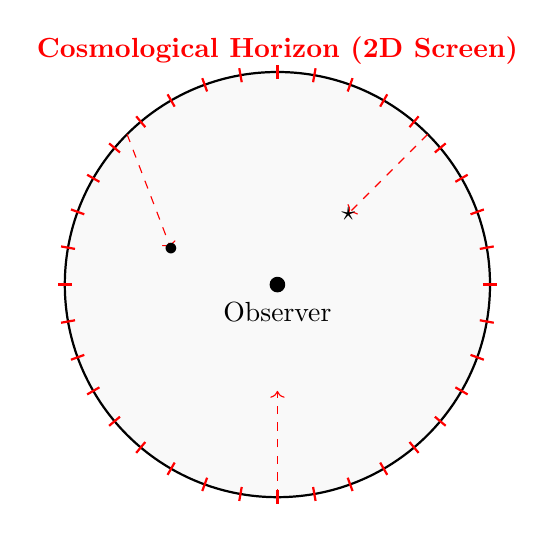
\begin{tikzpicture}[scale=0.9]
        % Horizon
        \draw[thick, fill=gray!5] (0,0) circle (3cm);
        \node[text=red] at (0,3.3) {\textbf{Cosmological Horizon (2D Screen)}};
        \node[circle, fill=black, inner sep=2pt, label=below:Observer] (O) at (0,0) {};
        
        % Projection
        \draw[dashed, ->, red] (45:3cm) -- (1,1);
        \draw[dashed, ->, red] (135:3cm) -- (-1.5, 0.5);
        \draw[dashed, ->, red] (270:3cm) -- (0, -1.5);
        
        % Objects
        \node at (1,1) {$\star$};
        \node at (-1.5, 0.5) {$\bullet$};
        \node at (0, -1.5) {$\galaxy$}; 
        
        % Boundary Bits
        \foreach \angle in {0,10,...,360} {
            \draw[red, thick] (\angle:2.9cm) -- (\angle:3.1cm);
        }
    \end{tikzpicture}
    \caption{\textbf{Boundary Encoding.} 3D spacetime emergent from horizon data.}
\end{figure}

\section*{References}
\begin{enumerate}
    \item Bekenstein, J. D. (1973). Black holes and entropy. \textit{Physical Review D}, 7(8).
    \item Hawking, S. W. (1975). Particle creation by black holes. \textit{Comm. Math. Phys.}
    \item 't Hooft, G. (1993). Dimensional reduction in quantum gravity. arXiv:gr-qc/9310026.
    \item Susskind, L. (1995). The world as a hologram. \textit{J. Math. Phys.}
    \item Maldacena, J. (1998). The large N limit of superconformal field theories. \textit{Adv. Theor. Math. Phys.}
    \item Pasterski, S., et al. (2023). Celestial holography. \textit{Rev. Mod. Phys.}
    \item Planck Collaboration. (2020). Planck 2018 results. VI. \textit{A\&A}.
    \item Event Horizon Telescope Collaboration. (2022-2025). First Sgr A* and M87 images.
\end{enumerate}

\vspace{1cm}
\begin{tcolorbox}
\textbf{ARG Research Disclaimer:} This document presents working hypotheses for scientific discussion. It does not claim medical, therapeutic, or commercial applications. Independent validation required.
\end{tcolorbox}

\vspace{1cm}
\begin{center}
    \line(1,0){250} \\
    \vspace{0.3cm}
    \small \copyright 2026 Alliance Research Group. Open Access. \\
    \url{ar-group.ai}
\end{center}

\end{document}